\chapter{The \texttt{IsoGene} Library in $R$}
\markchapter{IsoGene R} \label{chap: isogene}

\section{Introduction to \texttt{IsoGene} Package}
\label{sec: intro}

%R is a language and a free software environment for statistical
%computing and graphics. It is a GNU project (a complete Unix-like
%operating system developed in 1984, which is free software) which is
%similar to the S language and environment which was developed at
%Bell Laboratories (formerly AT\&T, now Lucent Technologies) by John
%Chambers and colleagues. R can be considered as a different
%implementation of S. There are some important differences, but much
%code written for S runs unaltered under R.

%$R$ provides a wide variety of statistical and graphical techniques,
%and is highly extensible. It is an integrated suite of software
%facilities for data manipulation, calculation and graphical display.
%$R$, like $S$, is designed around a true computer language, and it
%allows users to add additional functionality by defining new
%functions. $R$ is an environment within which statistical techniques
%are implemented so that it can be extended (easily) via packages.
%The packages supplied with the $R$ distribution and many more are
%available through the Comprehensive R Archive Network (CRAN) family
%of Internet sites covering a very wide range of modern statistics.



%In this chapter, we present an $R$ package called \texttt{IsoGene}
%to implement the statistical methods discussed by Lin \textit{et
%al.}\ (2007), where the primary interest is testing for a monotonic
%relationship between gene-expressions and doses in a microarray
%experiment. %Lin \textit{et al.} discussed the five test statistics,
%including the global likelihood ratio test ($\bar{E}^2_{01}$,
%Bartholomew 1961, Barlow \textit{et al.} 1972, and Robertson
%\textit{et al.} 1988), Williams (1971, 1972), Marcus (1976), M (Hu
%\textit{et al.} 2005) and the modified M (Lin \textit{et al.} 2007)
%and using permutations to obtain the raw $p$-values of the test
%statistics and adjusting $p$-values using BH (Benjamini and Hochberg
%1995) and BY (Benjamini and Yekutilie 2001) procedures controlling
%FDR.


The main IsoGene package functions are \texttt{IsoRawp()} and
\texttt{IsoTestBH()}, which calculate the raw $p$-values using
permutations and adjust them using the BH- and BY-FDR procedures.
The supporting functions \texttt{IsoGene1()} and \texttt{IsoGenem()}
are used to calculate the five test statistics from isotonic
regression for one gene and all the genes, respectively. On the other hand,
the SAM procedure is also implemented to reduce some computational time as
compared to the permutation method. The main function of the SAM is \texttt{IsoTestSAM()},
with supporting functions \texttt{Isofudge(), IsoGenemSAM(), Isoqqstat(), Isoallfdr(), Isoqval()}.
The remaining functions \texttt{IsopvaluePlot(), IsoBHPlot(), IsoSAMPlot()
IsoPlot1()} and \texttt{IsoPlot2()} are used to display the data and
to show the results of testing procedures.

\section{Testing for Trends: Testing Procedures, Multiplicity and Resampling-based Inference}
\subsection{Resampling-based Multiple Testing}

\sloppy{For adjusting for multiple testing, only the BH-FDR procedure
(Benjamini and Hochberg 1995) and BY-FDR procedure (Benjamini and
Yekutieli 2001) are considered in library \texttt{IsoGene()}. The
matrix of the values of the test statistics for each gene and
permutation is referred as the permutation matrix under the null
distribution (see Section 3.2.2).}

This matrix is used to calculate the one-sided $p$-values for the
inference. In the first step the one-sided raw (unadjusted for
multiple testing) $p^{Up}$-values are calculated using (\ref{p1}) or
(\ref{p2}) based on the test statistic $T^{Up}$.

\begin{equation}
P_i=\frac{\#(b: t_{ib} \ge t_{i})}{B-1}, \label{p1}
\end{equation}
where $t_i$ is the observed test statistic for gene $i$.

\begin{equation}
P_i=\frac{\sum_{b=1}^{B} \sum_{j=1}^{m} (t_{jb}\ge
t_{i})}{(B-1) \times m} \label{p2}.
\end{equation}

For $p^{Down}$-values, expect of $\bar{E}^2_{01}$, for which the
test statistic value $t_i$ is always between 0 and 1 and can be
obtained in the same way as $p^{Up}$-values,
\[p^{Down}=\#(b:t_{ib} \le t_{i})/B\; \mbox{or}\; p^{Down}=\sum_{b=1}^{B}
\sum_{j=1}^{m} (t_{jb} \le t_{i})/(B \times m)\] should be used
with $t_{ib}$ and $t_{jb}$ the test statistic values obtained for
gene $i$ and $j$ from permutation $b$. This is because under the
decreasing trend, we reject the four test statistics (namely,
Williams', Marcus', the $M$ and modified $M$) with large negative
values.

Based on the $p$-values, various methods adjusting the type I error
can be applied, such as the Bonferroni, Holm, Hochberg, and BH-FDR
and BY-FDR (Reiner \textit{et al.}\ 2003 and Ge \textit{et al.}\
2003).

\subsection{Significance Analysis of Microarray (SAM)}

SAM (Tusher \textit{et al.}\ 2001, Lin \textit{et al.}\ 2008) is a procedure widely used in the
microarray setting. SAM is a testing procedure, which estimates the
FDR by using permutations under the assumption that all null
hypotheses are true. The procedure consists of three components: (1)
the adjusted test statistics, (2) an approximation of the
distribution of the test statistics based on permutations, and (3)
the control of the FDR.

For a two-group setting, the modified test statistic in SAM is given
by,

\begin{equation}
t_{k}^{SAM}= \frac{\bar{x}_{k}-\bar{x}_{l}} {s_{k}+s_{0}},
\label{ttestSAM}
\end{equation}

where \[ \bar{x}_{l}=\frac{\Sigma_{j=1}^{n_{l}} x_{jl}}{n_{l}},\;\;
\bar{x}_{k}=\frac{\Sigma_{j=1}^{n_{k}} x_{jk}}{n_{k}},\;\;\]
\[s_{k}=\sqrt{\left (\frac{1}{n_{k}}+\frac{1}{n_{l}} \right )
{\frac{\Sigma_{j=1}^{n_{k}}
   (x_{jk}-\bar{x}_{jk})^2+\Sigma_{j=1}^{n_{l}}
   (x_{jl}-\bar{x}_{jl})^2}{n_{k}+n_{l}-2}}},
   \]
and $s_0$ is the fudge factor which is estimated from the data and
is discussed later, $k$ and $l$ are the index of the two groups of
array, and $j$ is the index of the array.

For $F$-type test statistic, such as $\bar{E}_{01}^2$, the modified test
statistic is given by,
\begin{equation}
\bar{E}_{01}^{2SAM}= \frac{\sqrt{\hat{\sigma}^2_{H_0}-\hat{\sigma}^2_{H_1}}} {\sqrt{\hat{\sigma}^2_{H_0}}+s_{0}},
\label{ttestSAM}
\end{equation}






SAM requires that the test statistic for each permutation is sorted
for all the genes, such that the first row of the sorted matrix is
the minimum test statistic across permutations, and the last row is
the maximum, i.e.,
\[\T^{SAM}= \left (
\begin{array}{llll}
t_{(1)1} & t_{(1)2} & \dots & t_{(1)B}\\
t_{(2)1} & t_{(2)2} & \dots & t_{(2)B}\\
.    & .    &.      & .     \\
.    & .    &.      & .     \\
.    & .    &.      & .     \\
t_{(m)1} & t_{(m)2} & \dots & t_{(m)B}\\
\end{array}
\right ).
\]

In $\T^{SAM}$, each element $t_{(i)b}$ is the sorted test statistic
for gene $i$ in permutation $b$. The expected values of the observed
ordered statistics are approximated by the means of the rows of
$\T^{SAM}$, given by $\bar{t}_{(1)}^{SAM}, \bar{t}_{(2)}^{SAM},
\dots, \bar{t}_{(m)}^{SAM}$ that are constructed in the following
way:
\[
\T^{SAM}= \left (
\begin{array}{llll}
t_{(1)1} & t_{(1)2} & \dots & t_{(1)B}\\ \hline t_{(2)1}
& t_{(2)2} & \dots & t_{(2)B}\\ \hline .    & . &.      & .
\\ \hline .    & .    &.      & .     \\ \hline . & .    &.      & .
\\ \hline
t_{(m)1} & t_{(m)2} & \dots & t_{(m)B}\\
\end{array}
\right ) \Rightarrow \left (
\begin{array}{l}
\frac{1}{B}\sum_{b=1}^{B}t_{(1)b} \\
\frac{1}{B}\sum_{b=1}^{B}t_{(2)b} \\
.                                     \\
.                                     \\
.                                     \\
\frac{1}{B}\sum_{b=1}^{B}t_{(m)b} \\
\end{array}
\right ) = \left (
\begin{array}{l}
\bar{t}_{(1)}^{SAM} \\
\bar{t}_{(2)}^{SAM} \\
.                                     \\
.                                     \\
.                                     \\
\bar{t}_{(m)}^{SAM} \\
\end{array}
\right ).
\]

%\noindent \textbf{SAM Procedure}

The SAM procedure proposed by Tusher \textit{et al.}\ (2001) is as
follows:

\begin{enumerate}

\item Compute order statistics $t_{(1)}^{SAM} \le t_{(2)}^{SAM} \le
\dots \le t_{(m)}^{SAM}$.

\item Compute the permutation matrix $\T^{SAM}$.

\item Calculate the expected test statistics
$\bar{t}_{(1)}^{SAM},\bar{t}_{(2)}^{SAM},\dots,\bar{t}_{(m)}^{SAM}$.

\item Plot the $t_{(1)}^{SAM} , t_{(2)}^{SAM}, \dots , t_{(m)}^{SAM}$
values versus the
$\bar{t}_{(1)}^{SAM},\bar{t}_{(2)}^{SAM},\dots,\bar{t}_{(m)}^{SAM}$
values (SAM plot).

\item For a fixed threshold $\Delta$, starting at the origin, and
moving up to the right, find the first $i=i_1$ such that
$t_i^{SAM}-\bar{t}_{i}^{SAM} > \Delta$. All genes, for which
$t_i^{SAM}$ $>$ $t_{i1}^{SAM}$, are called ``significant positive".
Similarly, start at origin, move down to the left and find the first
$i=i_2$ such that $\bar{t}_{2}^{SAM}-t_i^{SAM}> \Delta$. All genes,
for which $t_i^{SAM}$ $<$ $t_{i2}^{SAM}$, are called ``significant
negative". For each $\Delta$ define the upper cut-point
C$_{up}(\Delta)$ as the smallest $t_i^{SAM}$ among the significant
positive genes, and similarly define the lower cut-point
C$_{low}(\Delta)$.

\item For a grid of $\Delta$ values, compute the total number of
significant genes (from step 5), and the median number of falsely
called genes, i.e., the median number of values among each of the
$B$ sets of $t_{ib}$ , $i=1,2,\dots,m$ that fall above cut-point
C$_{up}(\Delta)$ and below cut-point C$_{down}(\Delta)$.
Similarly, compute the $90$th percentile of the number of falsely
called genes.

\item Estimate $\pi_0$, the proportion of truly non-differentially
expressed genes in the data set, as follows:

\begin{enumerate}

\item Compute the first and third quantiles of the permuted
$t^{SAM}$ values, denoted as $q25$ and $q75$ (the $t_i^{SAM}$ are
the values for the original data set; there are $m$ such values).

\item Compute  $\hat{\pi}_0 = \# \{ t_{i} \in (q25, q75)\} / (.5m)$.

\item Let $\hat{\pi}_0 = min (\hat{\pi}_0 , 1)$.
\end{enumerate}

\item  The median and the $90$th percentile of the number of falsely
called genes from step 6, are multiplied by $\hat{\pi}_0$,

\item Pick a $\Delta$ and the corresponding number of significant genes.


\item The FDR is estimated by the median (or the $90$th percentile) of the
number of falsely called genes divided by the number of significant
genes.


%\item $q$-value is the lowest FDR, at which a gene is called
%``significant". It resembles the $p$-value, but is adapted to the
%analysis of a large number of genes. Note that as $ t^{SAM}_i> 0$
%increases, the corresponding $q$-value decreases.

\end{enumerate}


\noindent \textbf{Estimation of the SAM Fudge Factor $s_0$}

In the procedure described above, a fudge factor $s_0$ in the
denominator of the test statistic~(\ref{ttestSAM}) is used. It is
calculated as the percentile of the gene-wise standard error
distribution that minimizes the coefficient of variation (CV) of the
test statistics. This modification is used to overcome bias for
genes with expressions close to zero, which have a large value of
the test statistic due to a small sample variance. By using an
inflated standard error, SAM addresses the problem of the dependence
of the value of the test statistic on the variance of expression
levels for a particular gene. The calculation of $s_0$ is as
follows:

\begin{enumerate}

\item Let $s_{\alpha}$ be the $\alpha \cdot 100\%$ percentile of $s_i$ values.
Let $t_i^{\alpha}= (\bar{X}_{1}-\bar{X}_{0})/(s_i+s_{\alpha})$.

\item Compute the 100 centiles of the $s_i$ values, denoted by $q_1 <
q_2\dots < q_{100}$.

\item For $\alpha \in (0, 0.05, 0.10, \dots, 1.0)$

\begin{enumerate}

\item compute $\nu_j= \mbox{MAD}(t_i^{\alpha}|s_i \in
[q_j,q_{j+1})),j=1,2,\dots,m$, where \mbox{MAD} is the median
absolute deviation from the median, divided by .64;

\item compute $cv(\alpha)=$ coefficient of variation of the $\nu_j$
values.

\end{enumerate}

\item Choose $\hat{\alpha}=argmin[cv(\alpha)]$, i.e.,
$\hat{\alpha}$ is the quantile of the standard error that minimizes
the coefficient of variation of the SAM test statistics.

\item Compute $\hat{s}_0=s_{\hat{\alpha}}$.

\end{enumerate}




\section{Using \texttt{IsoGene} Library}

\subsection{Data Example}

The data used for the analysis presented below are outcome of a dose-response microarray experiment
consisting of four dose levels. Three microarray samples are available at each dose level (hence, in total
gene expression was measured for 12 arrays). Each array consists of 16,998 genes.

A dataframe with the log2 transformed gene intensities is loaded
into $R$ environment. The first ten genes and first six samples are
displayed, where the row names of the genes show the probe ID,
\texttt{X1, X1.1 and X1.2} are the three arrays for dose zero, while
\texttt{X2, X2.1 and X2.2} are the arrays for the first dose. The dataframe is loaded suing the function \texttt{load()},
\begin{center}
\begin{boxit}
\begin{verbatim}
> load("data.Rdata")
\end{verbatim}
\end{boxit}
\end{center}
A printout of the first 10 lines is given below.
\begin{center}
\begin{boxit}
\begin{verbatim}
> data[1:10,1:6]
                 X1     X1.1     X1.2       X2     X2.1     X2.2
31637_s_at 6.923109 7.024719 7.170328 7.219297 7.076908 7.404949
32402_s_at 5.107275 5.092935 5.255918 5.312913 4.893855 4.596591
33646_g_at 5.913526 6.026197 5.141728 5.828770 5.269202 5.461664
34063_at   4.919469 4.908159 3.500307 4.814068 4.139949 4.278321
33494_at   6.002091 5.878718 5.777668 6.214799 5.895586 6.163291
34031_i_at 7.162715 7.294693 6.903935 7.223069 6.972928 7.412160
34449_at   4.049696 4.748409 3.845498 4.780287 4.076589 4.300242
34478_at   3.191931 4.326571 3.771206 3.570291 2.179324 3.988911
35436_at   6.487708 6.285804 6.229814 6.109103 6.340837 5.931840
36711_at   6.695870 6.687039 6.652153 6.503670 6.387794 6.698711
\end{verbatim}
\end{boxit}
\end{center}

\subsection{Loading the Library}

\sloppypar {To load the \texttt{IsoGene} package into $R$, a binary
zip-package of \texttt{IsoGene} program (for Windows) needs to be
installed. \texttt{IsoGene} library requires $R$ packages
\texttt{Multtest} and \texttt{ff}, which need to be installed as
well. Once the packages are installed, they are available for use
after being loaded in memory, which is usually done by the user:}
\begin{center}
\begin{boxit}
\texttt{> library(IsoGene)}
\end{boxit}
\end{center}
The functions included in the package can be listed using the $R$
help system:
\begin{center}
\begin{boxit}
\texttt{> help(IsoGene)}
\end{boxit}
\end{center}
%\begin{figure}[!h]
%\centering
%{\subfigure{\resizebox{.89\textwidth}{!}{\includegraphics{D:/Data/Ph.Dthesis/Figures/IsoGeneLib/page1.eps}}}\\
%\subfigure{\resizebox{.9\textwidth}{!}{\includegraphics{D:/Data/Ph.Dthesis/Figures/IsoGeneLib/page2.eps}}}
%} \caption{\em{The main help file of IsoGene package.}}
%\label{IsoGeneHelp}
%\end{figure}



%\begin{figure}[!h]
%\centering
%{\includegraphics[width=.6\textwidth]{IsoGenehelp.eps}}
%\caption{\em{The main help file of IsoGene package.}}
%\label{IsoGeneHelp}
%\end{figure}


%The help file of \texttt{IsoGene} package is shown in
%Figure~\ref{IsoGeneHelp}.
First, \texttt{IsoPlot1()} and \texttt{IsoPlot2()} can be used to
explore the data. Second, \texttt{IsoGene1()} and
\texttt{IsoGenem()} can be used to calculate the test statistics.
Third, \texttt{IsoRawp()} provides the output for two-sided or
one-sided $p$-values ($p^{Up}$ or $p^{Down}$). Based on the
$p$-values obtained, one can choose one test statistic and
multiplicity adjustment method for inference by using
\texttt{IsoTestBH()}. Finally, \texttt{IsopvaluePlot()} can be
useful for examining both of $p^{Up}$- or $p^{Down}$-values, and in
particularly, as a post hoc procedure it can be used to examine
genes with both small $p^{Up}$- and $p^{Down}$-values.


\section{The \texttt{IsoGene} Functions}
\subsection{Quick Start}
The first stage of the analysis (which is also the time consuming stage) consists of permutations under the null hypothesis in order to obtain the distribution of the test statistic under the null hypothesis. Note that, by default, all five test statistics discussed above are calculated. The function \texttt{IsoRawp()} is used to perform the permutation. A general call of the function \texttt{IsoRawp()} has the form of
\begin{center}
\begin{boxit}
\begin{verbatim}
IsoRawp(x, data, niter=1000, seed=1234)
\end{verbatim}
\end{boxit}
\end{center}
Here, \texttt{x} is a vector which contains the dose levels and \texttt{data} is the R object, which contains the information about gene expression and genes names. Once the permutation stage is completed, the FDR adjusted $p$-values can be obtained using function \texttt{IsoTestBH()}. The function calculates the adjusted p values for each statistic using either the BH-FDR or BY-FDR for multiplicity adjustment. The user can specify one of the five test statistics discussed above, or use the default call, in the later case adjusted $p$-values for all test statistics will be calculated. A general form of the \texttt{IsoTestBH()} has the form
\begin{center}
\begin{boxit}
\begin{verbatim}
IsoTestBH(rp, FDR=c(0.05,0.1), type=c("BH","BY"),
stat=c("E2","Williams","Marcus","M","ModifM"))
\end{verbatim}
\end{boxit}
\end{center}
Note that \texttt{rp} is an R object, which contains all the output produced by the function \texttt{IsoRawp()}.\newline In what follows we illustrate in more details the use of the functions of the \texttt{IsoGene} library.
\subsection{Exploring the Data}
\texttt{IsoPlot1()} and \texttt{IsoPlot2()} are two plotting
functions that can be used to explore the data. Scatterplots for the
second gene in the dataset (\texttt{data[2,]}) can be produced by
\begin{center}
\begin{boxit}
\begin{verbatim}
> x <- c(rep(1,3), rep(2,3), rep(3,3), rep(4,3))
> gene1 <- data[2,]
> par(mfrow=c(1,2))
> IsoPlot1(x, y=gene1)
> IsoPlot2(x, y=gene1)
\end{verbatim}
\end{boxit}
\end{center}

\begin{figure}[!h]
\centering
{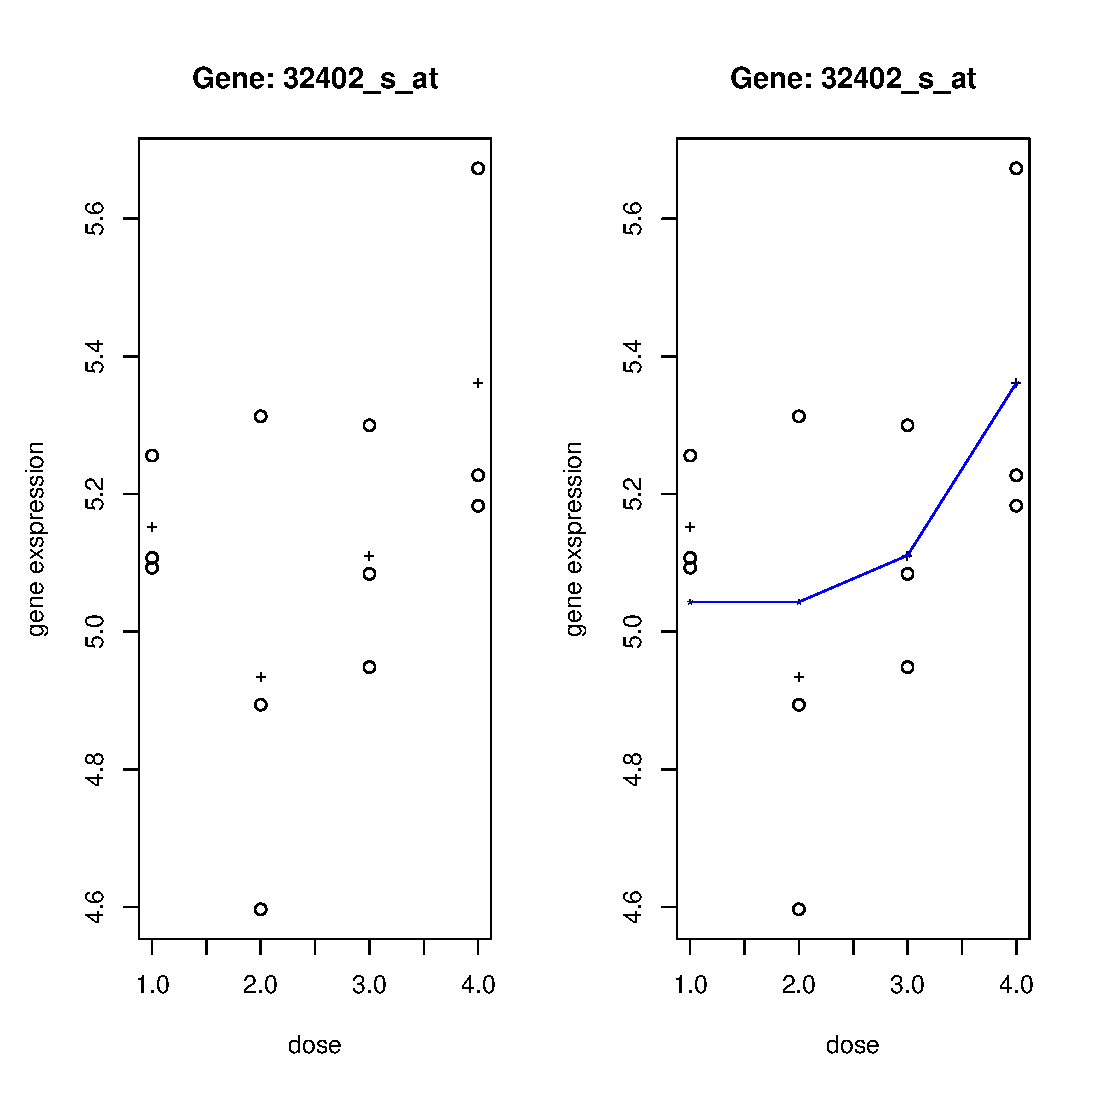
\includegraphics[width=.6\textwidth]{exgene.eps}}
\caption{\em{The data points are plotted as circles, while sample
means as pluses. The right panel additionally plots the fitted
increasing isotonic regression model (blue solid line).}}
\label{exgene}
\end{figure}


The left panel in Figure~\ref{exgene} shows the original data points
(as circles) and sample means (as pluses) for each dose. The right
panel in Figure~\ref{exgene} shows the increasing isotonic
regression model (blue solid line) fitted on the data. The fitted
monotonic line does not indicate the significance of the test, but
simply shows a more likely increasing (or decreasing) trend.


\subsection{Calculating the Test Statistics}

The five test statistics described in Chapter 2 can be obtained by
using the function \texttt{IsoGene1()} for a single gene and using
the function \texttt{IsoGenem()} for all the genes simultaneously.
The following $R$ codes illustrate the input and output generated by
these two functions:
\begin{center}
\begin{boxit}
\texttt{
> stat1 <- IsoGene1(x, gene1)}
\end{boxit}
\end{center}
The object \texttt{stat1} contains the information about the five test statistics and the direction for which the likelihood is maximizes.
\begin{center}
\begin{boxit}
\texttt{
> stat1\\
\$ E2.up [1] 0.2010957\\
\$ Williams.up [1] 0.6712589\\
\$ Marcus.up [1] 1.3646790\\
\$ M.up [1] 1.0004640\\
\$ ModM.up [1] 1.0611520\\
\$ E2.dn [1] 0.0098105\\
\$ Williams.dn [1] -0.2850243\\
\$ Marcus.dn [1] -0.2850243\\
\$ M.dn [1] -0.1876899\\
\$ ModM.dn [1] -0.2098437\\
\$ direction [1] "u" }
\end{boxit}
\end{center}

The first 10 objects are the values calculated for the five test
statistics under increasing and decreasing trends. The last object
indicates the higher likelihood of isotonic regression with ``u"
meaning a increasing trend or ``d" meaning a decreasing trend.


We use the first 10 genes as an example to illustrate the use of
function \texttt{IsoGenem()}:
\begin{center}
\begin{boxit}
\begin{verbatim}
> statm <- IsoGenem(x, data[1:10,])
\end{verbatim}
\end{boxit}
\end{center}

\begin{center}
\begin{boxit}
\begin{verbatim}
> statm
$E2.up
         2          3          4          5          6
0.00000000 0.20109571 0.50774178 0.24835414 0.00000000
         7          8          9         10         11
0.16263545 0.43080221 0.00000000 0.06367646 0.00000000
$Williams.up
 [1] -1.1298186  0.6712589  2.4888850  0.8911883 -0.6520746
 [6]  0.5582301  2.1412458 -0.5774471  0.8895008 -1.6655641
$Marcus.up
 [1] 0.0000000 1.3646791 2.4888850 1.3929232 0.0000000
 [6] 1.4262255 2.1412458 0.0000000 0.8895008 0.0000000
$M.up
 [1] 0.0000000 1.0004635 2.0194520 0.9386711 0.0000000
 [6] 0.7196721 1.6954778 0.0000000 0.4960717 0.0000000
$ModM.up
 [1] 0.0000000 1.0611518 2.1419523 1.0494662 0.0000000
 [6] 0.8046179 1.7983258 0.0000000 0.5261635 0.0000000
$E2.dn
          2           3           4           5           6
0.275992755 0.009810531 0.000000000 0.002919082 0.139779913
          7           8           9          10          11
0.079338232 0.000000000 0.099457466 0.124447675 0.456682221
$Williams.dn
 [1] -1.66138158 -0.28502430  1.72265475  0.06394548
 [5] -1.10255870 -1.01756814  1.31114235 -0.76992952
 [9]  0.12749125 -3.83085270
$Marcus.dn
 [1] -1.6613816 -0.2850243  0.0000000 -0.1743749 -1.1025587
 [6] -1.1502473  0.0000000 -0.7699295 -1.0674972 -3.8308527
$M.dn
 [1] -1.2705909 -0.1876899  0.0000000 -0.1020262 -0.9002354
 [6] -0.5535348  0.0000000 -0.6266432 -0.6156540 -2.0821512
$ModM.dn
 [1] -1.3476651 -0.2098437  0.0000000 -0.1140688 -0.9002354
 [6] -0.6188707  0.0000000 -0.7006084 -0.6883221 -2.2084548
$direction
  2   3   4   5   6   7   8   9  10  11
"d" "u" "u" "u" "d" "u" "u" "d" "d" "d"
\end{verbatim}
\end{boxit}
\end{center}

The output from \texttt{IsoGenem()} has the same structure as the one
for \texttt{IsoGene1()}, but each object contains the values of the
test statistics and the likely direction of the isotonic regression
model for all the genes.


\subsection{Obtaining Raw $p$-values}

As discussed above, we use permutations to obtain the raw $p$-values
for the five test statistics. The function \texttt{IsoRawp()} can be
used in the following way:
\begin{center}
\begin{boxit}
\begin{verbatim}
> rawp <- IsoRawp(x=x, y=data, niter=1000, seed=1234)
\end{verbatim}
\end{boxit}
\end{center}


The four arguments in this function need to be specified, with no
default pre-specified values. \texttt{x} is the explanatory variable
indicating the dose levels for all the samples in the data.
\texttt{data} is the data frame of the gene expression.
\texttt{niter} defines the number of permutations used to
approximate the null distribution and \texttt{seed} determines the
random seed used to generate the permutations. The output item
\texttt{rawp} contains four objects with $p$-values for the five
test statistics: the first one contains the two-sided $p$-values,
the second contains the one-sided $p$-values, the third contains
$p^{Up}$-values, and the last one contains $p^{Down}$-values. Below
we print a part of the object with two-sided $p$-values for illustration:
\begin{center}
\begin{boxit}
\texttt{
> rawp.twosided=rawp[[1]]}
\end{boxit}
\end{center}
The first 10 rows in of the object \texttt{rawp.twosided} are
\begin{center}
\begin{boxit}
\texttt{
> rawp.twosided[1:10,]\\\\
   Probe.ID      E2  Williams  Marcus  M   ModM\\
1  31637\_s\_at 0.000 0.000  0.000 0.000 0.000\\
2  32402\_s\_at 0.129 0.225  0.124 0.123 0.125 \\
3  33646\_g\_at 0.003 0.004  0.003 0.003 0.002\\
4  34063\_at    0.487 0.379  0.500 0.467 0.474\\
5  33494\_at    0.071 0.185  0.035 0.063 0.064\\
6  34031\_i\_at 0.082 0.220  0.086 0.103 0.086\\
7  34449\_at    0.357 0.445  0.432 0.400 0.391\\
8  34478\_at    0.472 0.516  0.535 0.518 0.511\\
9  35436\_at    0.151 0.116  0.148 0.150 0.140 \\
10 36711\_at    0.000 0.000  0.000 0.000 0.000 \\}
\end{boxit}
\end{center}
The first output object from \texttt{rawp} is a matrix with six
columns, where the first column indicates the probe ID. Columns from
the second to the sixth are $p$-values for each of the five test
statistics, respectively. The remaining three output objects
(\texttt{rawp}[[2]], \texttt{rawp}[[3]], \texttt{rawp}[[4]]) are
structured in the same way.


\subsection{Plot of $p$-values for a Single Gene}

For a single gene, the function \texttt{IsopvaluePlot()} can be used
to show the $p^{Up}$ and $p^{Down}$-values for a given test
statistic:
\begin{center}
\begin{boxit}
\begin{verbatim}
IsopvaluePlot(x, y, niter, seed, stat = c("E2", "Williams",
"Marcus", "M", "ModifM"))
\end{verbatim}
\end{boxit}
\end{center}
We use one gene as an example to illustrate how $p^{Up}$ and
$p^{Down}$-values (in the upper and lower panels of
Figure~\ref{expvalue}) are obtained. In Figure~\ref{expvalue}, the
observed test statistics are drawn as the dashed line, and the
values of the test statistics obtained from permutations are spread
over the x-axis. For this gene, the $p^{Up}$ is much smaller as
compared to the $p^{Down}$ since $T^{Up} \gg T^{Down}$, which
implies a possible increasing trend in the data.
\begin{center}
\begin{boxit}
\begin{verbatim}
> gene1 <- data[2,]
> IsopvaluePlot(x, gene1, niter=1000, seed=123, stat="E2")
\end{verbatim}
\end{boxit}
\end{center}
%\begin{center}
%Figure~\ref{expvalue}-ABOUT HERE
%\end{center}


\begin{figure}[!h]
\centering
{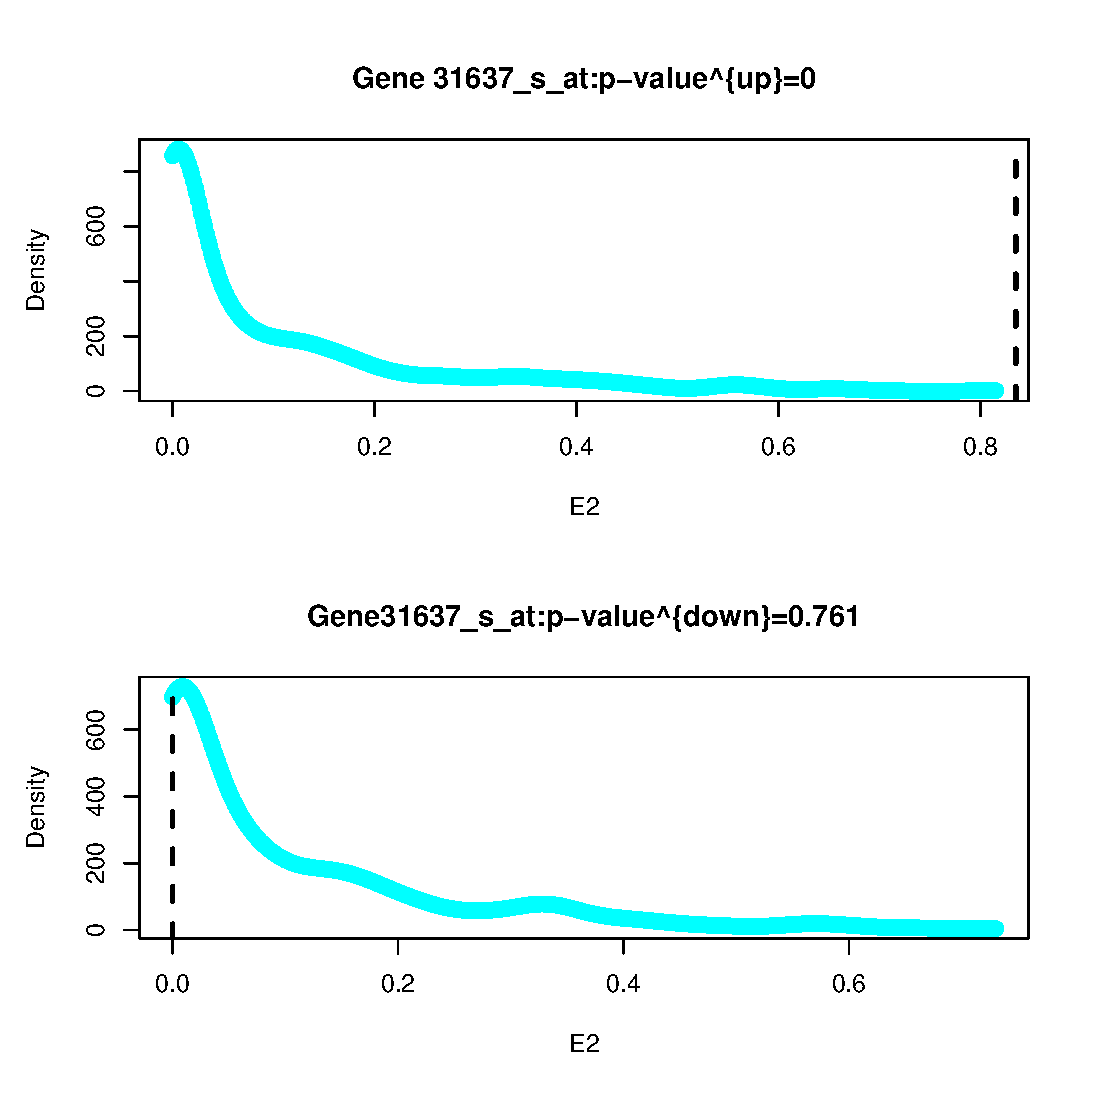
\includegraphics[height=10cm,width=12cm]{Isopval.eps}}
\caption{\em{The $p^{Up}$ and $p^{Down}$-values using
$\bar{E}_{01}^2$ for an example gene. The dashed line is the
observed test statistic value. In the upper panel, the dashed line
(at the right) is larger than most of the test statistics from
permutations, which results in a small $p^{Up}$-value. In the lower
panel, the dashed line (close to zero) is smaller than most of the
test statistics from permutations, which results in a large
$p^{Down}$-value.}} \label{expvalue}
\end{figure}



\subsection{BH/BY-FDR Procedures for Adjusting for Multiple Testing}

With the two-sided $p$-values, the user needs to select one of the
five test statistics, the FDR level, and the type of multiplicity
adjustment (BH-FDR or BY-FDR) to obtain the list of significant
genes:
\begin{center}
\begin{boxit}
\begin{verbatim}
IsoTestBH(rp, FDR=c(0.05,0.1), type=c("BH","BY"),
stat=c("E2","Williams","Marcus","M","ModifM"))
\end{verbatim}
\end{boxit}
\end{center}

The following example shows the use of the global likelihood ratio
test $\bar{E}^{2}_{01}$, the FDR level of 0.05 and the BH-FDR
procedure controlling the FDR: \\ \\
\begin{center}
\begin{boxit}
\begin{verbatim}
> E2.BH <- IsoTestBH(rawp.twosided, FDR=0.05, type="BH", stat="E2")
\end{verbatim}
\end{boxit}
\end{center}
The first 10 rows in the object \texttt{E2.BH} list the sorted row and adjusted p values for the $\bar{E}^{2}_{01}$ statistic.
\begin{center}
\begin{boxit}
\texttt{
> E2.BH[1:10,]\\
   Probe.ID    row.name raw p-values BH adjusted p values\\
1  31637\_s\_at   1        0.000          0.000000000\\
2  33646\_g\_at   3        0.003          0.015647131\\
3  36711\_at      10       0.000          0.000000000\\
4  37079\_at      12       0.001          0.007115111\\
5  37117\_at      13       0.011          0.042679297\\
6  37152\_at      14       0.003          0.015647131\\
7  38158\_at      29       0.003          0.015647131\\
8  38241\_at      30       0.000          0.000000000\\
9  39248\_at      35       0.003          0.015647131\\
10 39249\_at      36       0.008          0.033642751\\
}
\end{boxit}
\end{center}
Here we show only the first ten genes declared significant by using
$\bar{E}^{2}_{01}$ test. The output results in a matrix of five
columns: the first column indicates the probe ID, the second column
is the corresponding row number of significant genes in the original
dataset, the third column is the unadjusted/raw $p$-value, and the
last column is the adjusted $p$-value using the requested ``BH"
procedure. The order of the list of genes found significant is based
on the row number. Moreover, the function \texttt{IsoBHPlot()} can
be used to visualize the number of significant findings for the
BH-FDR and BY-FDR procedures for the specified test statistic:

\begin{center}
\begin{boxit}
\begin{verbatim}
IsoBHPlot(rp, FDR=c(0.05,0.1),
stat=c("E2","Williams","Marcus","M","ModifM"))
\end{verbatim}
\end{boxit}
\end{center}
Figure~\ref{IsoBHPlot} shows the unadjusted (solid blue line) and
the BH-FDR (dotted and dashed red line) and BY-FDR (dashed green
line) adjusted $p$-values for $\bar{E}^2_{01}$. It is obtained using
the function \texttt{IsoBHPlot()}:
\begin{center}
\begin{boxit}
\begin{verbatim}
> IsoBHPlot(rawp.twosided, FDR=0.05, stat="E2")
\end{verbatim}
\end{boxit}
\end{center}
%\begin{center}
%Figure~\ref{IsoBHPlot}-ABOUT HERE
%\end{center}


\begin{figure}[!h]
\centering
{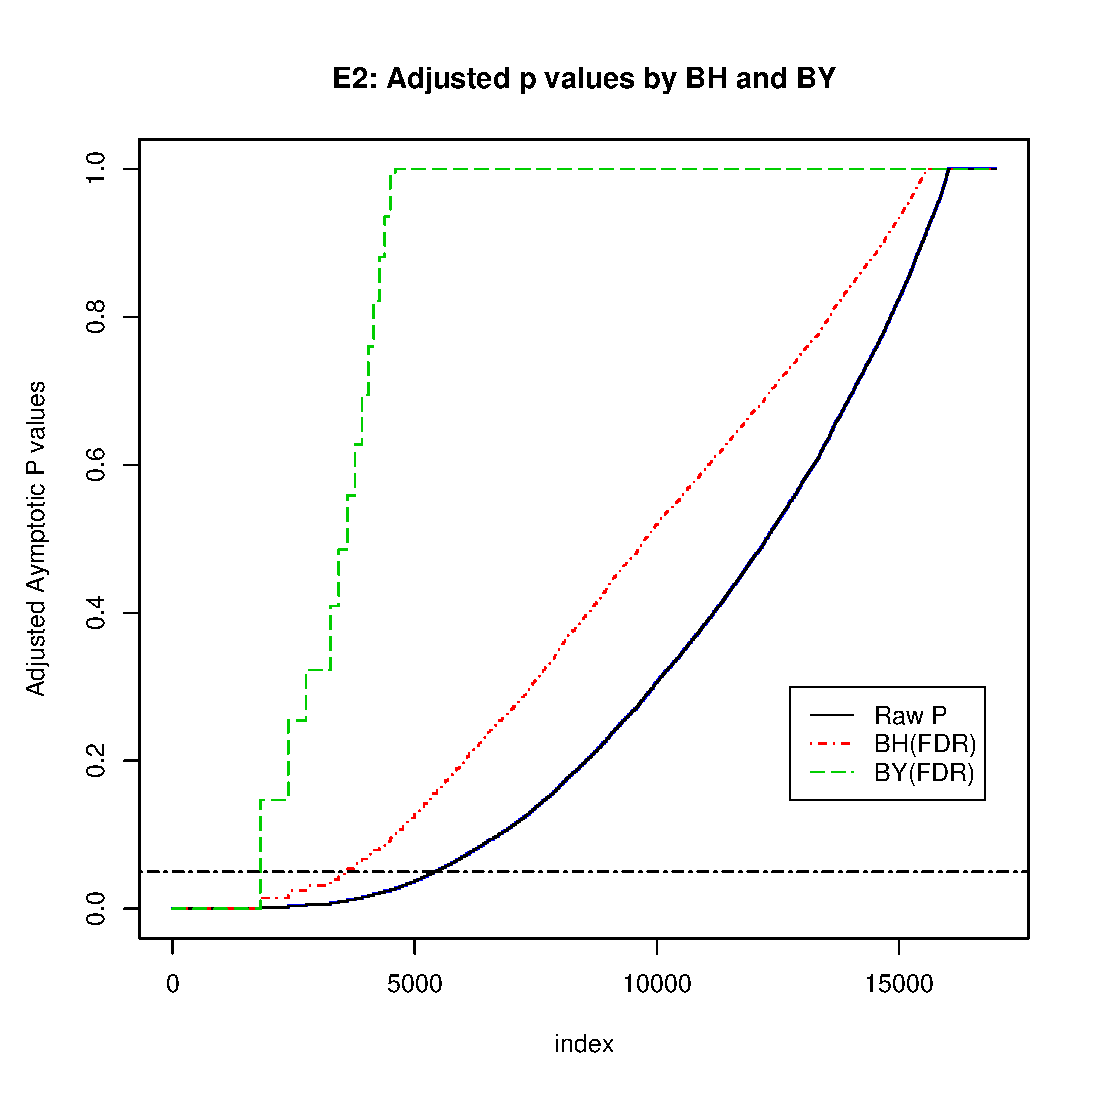
\includegraphics[width=.6\textwidth]{BHPlot1.eps}}
\caption{\em {The unadjusted (solid blue line), and the BH-FDR
(dotted and dashed red line) and BY-FDR (dashed green line) adjusted
$p$-values for $\bar{E}_{01}^2$.}} \label{IsoBHPlot}
\end{figure}



\section{Significance Analysis of Dose-response Microarray Data (SAM)}
In this library, we also implement the significance analysis of microarray (SAM) for testing
for the dose-response relationship under order restricted alternatives. The SAM procedure was proposed
by Tusher \textit{et al.}\ (2001) for finding differentially expressed genes by using permutations while controlling for
the FDR.

The main function for the SAM procedure is \texttt{IsoTestSAM()}. Within the main function, \texttt{Isofudge()}
calculates the fudge factor in the SAM test statistic, \texttt{IsoGenemSAM()} is used
to obtain the values of SAM test statistics, \texttt{Isoqqstat()} calculates the SAM test statistic
for the required number of permutations specified by users, \texttt{Isoallfdr()} obtains the delta table in the SAM procedure,
\texttt{Isoqval()} computes q-values of the SAM.  %And we can use \texttt{IsoSAMPlot}() to display outputs of the SAM.

The syntax of these function is as follows,
\begin{center}
\begin{boxit}
\begin{verbatim}
> Isofudge(x, y)
> IsoGenemSAM(x, y, fudge.factor)
> Isoqqstat(x, y, fudge=c(0,"pooled"), niter=100, seed=123)
> Isoallfdr(qqstat, ddelta, stat=c(E2","Williams","Marcus","M","ModifM"))
> Isoqval(delta, allfdr, qqstat, stat)
\end{verbatim}
\end{boxit}
\end{center}


We use the same data as above to obtain the fudge factor of the SAM procedure for
the five test statistics by using function \texttt{Isofudge()}.
\begin{center}
\begin{boxit}
\begin{verbatim}
> fudge.factor <- Isofudge(x, data)
> fudge.factor
\end{verbatim}
\end{boxit}
\end{center}

The output of this function gives a vector of five fudge factors for each of the test statistics.
\begin{center}
\begin{boxit}
\texttt{
[1] 0.0655931 0.2421966 0.1697765 0.1526049 0.1246253
}
\end{boxit}
\end{center}
Note that the fudge factor of the $\bar{E}_{01}^2$ is obtained based on the algorithm for F test
statistics given by Tusher \textit{et al.}\ (2001) and should be used with cautions. The performance of using
the fudge factor as compared to the $t$-type test statistics has not yet investigated in term of
power and control of the FDR. Therefore, it's advisable to use the fudge factor in the $t$-type test statistics.

\begin{center}
\begin{boxit}
\begin{verbatim}
> SAMtest.stat <- IsoGenemSAM(x, data, fudge.factor)
> names(SAMtest.stat)
\end{verbatim}
\end{boxit}
\end{center}
The output of the function gives
\begin{center}
\begin{boxit}
\texttt{
[1] "E2"        "Williams"  "Marcus"    "M"         "ModM"      "direction"
}
\end{boxit}
\end{center}

The following codes produce the values of the five test statistics for the first ten genes,

\begin{center}
\begin{boxit}
{ \small
\begin{verbatim}
> SAMtest.stat[[1]][1:10]
[1] 0.26447986 0.18999517 0.48012060 0.23728408 0.10796339
 0.14052809 0.42501333 0.09426217 0.11186881 0.41814965
> SAMtest.stat[[2]][1:10]
[1] -0.89438193  0.33788341  1.17016612  0.44809154 -0.37792503
0.16928575  1.40636038 -0.42466794  0.04789247 -1.26568858
> SAMtest.stat[[3]][1:10]
[1] -1.0376186  0.8067224  1.3904565  0.8226705 -0.4703604
0.5463295  1.5671898 -0.4904282 -0.4930563 -1.5825487
> SAMtest.stat[[4]][1:10]
[1] -0.8990584  0.6872440  1.2812581  0.6610949 -0.4531919
0.4158778  1.3448651 -0.4422525 -0.3838333 -1.2290796
> SAMtest.stat[[5]][1:10]
[1] -0.9924257  0.7608038  1.4288688  0.7586334 -0.4985868
0.4826826  1.4670386 -0.5074367 -0.4436651 -1.3792490
> SAMtest.stat[[6]][1:10]
2   3   4   5   6   7   8   9  10  11
"d" "u" "u" "u" "d" "u" "u" "d" "d" "d"
\end{verbatim}
}
\end{boxit}
\end{center}


To obtain the SAM test statistics for one of five test statistic values, for example, the modified M test,
with the required number of permutations specified by users and compute the
delta table in the SAM procedure, we can use function \texttt{Isoqqstat()} and \texttt{Isoallfdr()} as follows,
\begin{center}
\begin{boxit}
\begin{verbatim}
> qqstat <- Isoqqstat(x, data, fudge="pooled", niter=100, seed=123)
> dtable <-  Isoallfdr(qqstat, , stat="ModifM")
> dtable
     Ddelta FalsePositive50% FalsePositive90% Called FDR50% FDR90%
[1,]   0.03        9069.3117        9194.0314  16752 0.5414 0.5488
[2,]   0.05        8889.5505        9057.3462  16608 0.5353 0.5454
[3,]   0.07        8658.5881        8881.5364  16442 0.5266 0.5402
[4,]   0.09        8301.2919        8585.7932  16104 0.5155 0.5331
.
.
[40,]   0.81       46.7490          64.0573    926 0.0505 0.0692
---------------------------------------------------------------------
[41,]   0.83       41.7402          57.3232    872 0.0479 0.0657
---------------------------------------------------------------------
.
.
[115,]   2.31       0.0000          0.5565      20   0.0000 0.0278
[116,]   2.33       0.0000          0.5565      20   0.0000 0.0278
[117,]   2.35       0.0000          0.5565      20   0.0000 0.0278
[118,]   2.37       0.0000          0.5565      20   0.0000 0.0278
[119,]   2.39       0.0000          0.5565      19   0.0000 0.0293
\end{verbatim}
\end{boxit}
\end{center}
Note that in \texttt{Isoallfdr()}, ddelta is left blank, with default value taken
from the data, i.e., all the percentiles of the standard errors.
By fixing the 50\% FDR at 0.05, the corresponding delta value is 0.83
(marked in-between the dashed lines) as we obtain from the delta table above,
the number of differentially expressed genes are 872 with potential 42 genes as false positives.



\begin{center}
\begin{boxit}
\begin{verbatim}
> qval <- Isoqval(delta=0.83, allfdr=dtable, qqstat=qqstat,
stat="ModifM")
> dim(qval[[1]])
[1] 16998     3
> qval[[1]]
       [,1]      [,2]   [,3]
 1774   1773   -6.263922 0.0139
 7761   7760   -5.998759 0.0000
 1775   1774   -5.577230 0.0000
.
.
 8710   8709   7.21642443 0.0000
 16623 16622   8.00039508 0.0000
 5232  5131    8.78524604 0.0000
> dim(qval[[2]])
[1] 872    3
> qval[[2]]
       [,1]      [,2]   [,3]
 1774    1773  -6.263922 0.0139
 7761    7760  -5.998759 0.0000
 1774    1774  -5.577230 0.0000
.
.
 5521    5520   6.702022 0.0000
 8710    8709   7.216424 0.0000
 16623  16622   8.000395 0.0000
 5132    5131   8.785246 0.0000
\end{verbatim}
\end{boxit}
\end{center}

By specifying the desired delta value, delta table, and the user-defined test statistic in function \texttt{Isoqval()}, we can obtain
the q value of each gene from the SAM procedure. The first object of the output is the list of q values for
all the genes, ranking from the smallest test statistic value to the largest; while the second object is the list of q values
for the 872 differentially expressed genes, ranking from the smallest test statistic value to the largest. The first column of the output matrices is the row number of genes in
the data set, the second column is the observed modified M test statistic value, and the last column is the q value of the
SAM procedure for both objects.


Alternatively, we can use function \texttt{IsoTestSAM()} to summarize all the steps above and give results of a list of significant findings, which is the same second output of function \texttt{Isoqval()}.
\begin{center}
\begin{boxit}
\begin{verbatim}
> IsoTestSAM(x, y=data, fudge=c(0,"pooled"), niter=100, 
seed=123, FDR=0.05, stat=c("E2","Williams","Marcus","M","ModifM"))
\end{verbatim}
\end{boxit}
\end{center}

Specifying the same options as above in this function, we can obtain the list of significant genes as follows: the first column is the Probe.ID, the second column is the corresponding row numbers of the genes in the data set, the third column is the observed modified M SAM test statistics, the fourth column is the $q$ values of genes by using the SAM procedure. The last two columns gives additional information by calculating the $p$ values based on the SAM permutation matrix and adjusting these $p$ values using the BH-FDR procedure.
\begin{center}
\begin{boxit}
\begin{verbatim}
> IsoSAM.obj <- IsoTestSAM (x, y=data, fudge="pooled", 
niter=100, seed=123, FDR=0.05, stat="ModifM")
> IsoSAM.obj 
    Probe.ID row.number  stat.val qvalue       pvalue  adj.pvalue
1       1774       1773 -6.263922 0.0139 1.176609e-05 0.00937500
2       7762       7760 -5.998759 0.0000 1.176609e-05 0.00937500
3       1775       1774 -5.577230 0.0000 1.176609e-05 0.00937500
4       4625       4624 -5.384857 0.0000 1.176609e-05 0.00937500
.
.
869     5521       5520  6.702022 0.0000 1.176609e-05 0.00937500
870     8711       8709  7.216424 0.0000 5.883045e-06 0.00937500
871    16624      16622  8.000395 0.0000 0.000000e+00 0.00000000
872     5132       5131  8.785246 0.0000 0.000000e+00 0.00000000
\end{verbatim}
\end{boxit}
\end{center}

Finally, the graphic output of the SAM procedure can be produced using function \texttt{IsoSAMPlot()}.
\begin{center}
\begin{boxit}
\begin{verbatim}
> IsoSAMPlot(qqstat, allfdr, FDR=0.05, stat=c(E2","Williams",
"Marcus","M","ModifM"))
\end{verbatim}
\end{boxit}
\end{center}

This function requires the use of output from \texttt{Isoqqstat()} and \texttt{Isoallfdr()}, given a user-defined test statistic
and the FDR level to control. We still take the modified M test statistic for example, at the FDR of 0.05. There are four plots
yielded from the SAM procedure. Panel $a$ shows the FDR (either 50\% or 90\% (more stringent)) vs. $\Delta$, from which, user can choose the delta value with
the corresponding desired FDR. Panel $b$ shows the number of significant genes vs. $\Delta$, and panel $c$ shows the number of false positives (either 50\% or 90\%) vs. $\Delta$. Finally panel $d$ shows the observed vs. the expected (obtained from permutations) test statistics, in which the red dots are those genes called differentially expressed.
\begin{center}
\begin{boxit}
\begin{verbatim}
> IsoSAMPlot(qqstat=qqstat, allfdr=dtable, FDR=0.05, stat="ModifM")
\end{verbatim}
\end{boxit}
\end{center}

\begin{figure}[!h]
\centering
{\includegraphics[width=.7\textwidth]{SAMPlot.eps}}
\caption{\em {The SAM plots: a.Plot of the FDR vs. delta; b. Plot of number of significant genes vs. delta; c. Plot of
number of false positives vs. delta; d. Plot of observed vs. expected test statistics.}} \label{IsoBHPlot}
\end{figure}



\clearpage
\newpage


\section*{References}


\begin{list}{}{\setlength{\leftmargin}{.3in}\setlength{\itemindent}{-.2in}}

\item Agresti, A. (1997) \textit{Statistical Methods for the
Social Sciences}, Finlay.%

\item Barlow, R.E., Bartholomew, D.J.,
Bremner, M.J. and Brunk, H.D. (1972) \textit{Statistical inference
under order restriction}, New York: Wiley.%

\item Bartholomew, D.J. (1961) Ordered
tests in the analysis of variance, \textit{Biometrika}, \textbf{48},
325--332.%

\item Benjamini, Y. and Hochberg, Y.
(1995) Controlling the false discovery rate: a practical and
powerful approach to multiple testing. \textit{Journal of Royal
Statistical Soceity, Biostatistics}, \textbf{57}, 289--300.%


\item Benjamini, Y. and Yekutieli,
D. (2001) The control of the false discovery rate in multiple
testing under dependency. \textit{Annal of Statistics},
\textbf{29(4)}, 1165--1188.%


\item
Benjamini, Y. and Yekutieli, D. (2005) False Discovery
Rate-Adjusted Multiple Confidence Intervals for Selected Parameters.
{\em Journal of the American Statistical Association}, \textbf{100}, 71--81.%


\item Chuang-Stein, C. and Agresti, A. (1997) Tutorial in biostatistics:
A review of tests for detecting a monotone dose-response
relationship with ordinal response data, \textit{Statistics in
Medicine}, \textbf{16}, 2599--2618.%


\item Ge, Y., Dudoit, S. and Speed, P.T.
(2003) Resampling based multiple testing for microarray data
analysis,  \textit{technical report}, \textbf{633}, University of
Berkeley.%

\item Hu, J., Kapoor, M., Zhang, W.,
Hamilton, S.R. and Coombes, K.R. (2005) Analysis of dose response
effects on gene expression data with comparison of two microarray
platforms, \textit{Bioinformatics}, \textbf{21(17)}, 3524--3529.%

\item Lin, D., Shkedy, Z., Yekutieli, D., Burzykowki,
T., G\"{o}hlmann, H.W.H., De Bondt, A., Perera, T., Geerts, T.,
Bijnens, L. (2007a) Testing for trend in dose-response microarray
experiments: comparison of several testing procedures, multiplicity,
and resampling-based inference. \textit{Statistical Application in
Genetics and Molecular Biology}, \textbf{6(1)}, article 26.%

\item Lin, D., Shkedy, Z., Burzykowki, R., Ion,
T., G\"{o}hlmann, H.W.H., De Bondt, A., Perera, T., Geerts, T.,
Bijnens, L. (2008) An investigation on performance of Significance
Analysis of Microarray (SAM) for the comparisons of several
treatments with one control in the presence of small variance genes.
\textit{Biometrical Journal}, Multiple Comparison Problem, Special Issue,
\textbf{50(5)}, 801--823.%



\item Marcus, R. (1976) The powers of some tests of
the quality of normal means against an ordered alternative,
\textit{Biometrika}, \textbf{63}, 177--83.%

\item Reiner, A., Yekutieli, D. and
Benjamini, Y. (2003) Identifying differentially expressed genes
using false discovery rate controlling procedures.
\textit{Bioinformatics}, \textbf{19(3)}, 368--375.%

\item Robertson, T., Wright, F.T. and Dykstra, R.L. (1988) \textit{ Order restricted statistical inference}, Wiley.%



item Ruberg, S.J. (1995a) Dose response studies. I. Some design
considerations. \textit{Journal of Biopharmaceutical Statistics},
\textbf{5(1)}, 1--14.%

\item Ruberg, S.J. (1995b) Dose response studies. II. Analysis and
interpretation. \textit{Journal of Biopharmaceutical Statistics},
\textbf{5(1)}, 15--42.%

\item Tusher, V.G., Tibshirani, R. and
Chu, G. (2001) Significance analysis of microarrys applied to the
ionizing radiation response, \textit{Proceedings of the National
Academy of Sciences}, \textbf{98} , 5116--5121.%


\item Williams, D.A. (1971) A test for differences between treatment
means when several dose levels are compared with a zero dose
control, \textit{Biometrics}, \textbf{27}, 103--117.%

\item Williams, D.A. (1972) The comparision of several dose levels
with a zero dose control, \textit{Biometrics}, \textbf{28},
519--531.%


\end{list}




